\documentclass[11pt]{beamer}
\usepackage[utf8]{inputenc}
\usepackage[T1]{fontenc}
\usetheme{default}
\usepackage{tikz}
\usetikzlibrary{overlay-beamer-styles}


\begin{document}



\begin{frame}[t]{Tree demo} % ================================================================

\begin{onlyenv}<+->
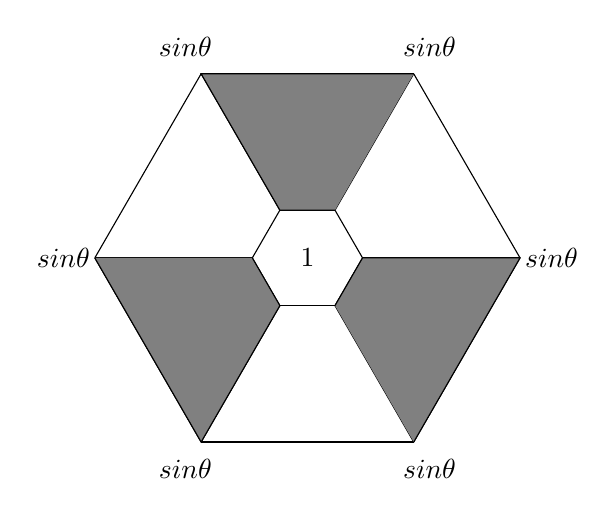
\begin{tikzpicture}
   \newdimen\R
   \R=2.7cm
   
    \newdimen\r
   \r=0.7cm
%   \draw (0:\R) \foreach \x in {60,120,...,360} {  -- (\x:\R) };
\node[rectangle]{1};
\foreach \x in {60,120,...,360}{
    \draw (\x:\R)  --  (\x+60:\R) ;
    \draw (\x:\r)  --  (\x+60:\r) ;
    \draw (\x:\r)  --  (\x:\R);
    
    };
    
    \node[visible on=<1->]  at  (60:3.1cm){$sin\theta$};
    \node[visible on=<2->]   at (120:3.1cm){$sin\theta$};
    \node[visible on=<3->]   at (180:3.1cm){$sin\theta$};
    \node[visible on=<4->]   at (240:3.1cm){$sin\theta$};
    \node[visible on=<5->]   at (300:3.1cm){$sin\theta$};
    \node[visible on=<6->]   at (360:3.1cm){$sin\theta$};
    
  \foreach \x in {60, 180, 300}{
    \draw[fill=gray] (\x:\r)--(\x+60:\r)--(\x+60:\R)--(\x:\R);
  };
    
  
%   \foreach \x/\l/\p in
%      { 60/{(2,3,1)}/above,
%       120/{(2,1,3)}/above,
%       180/{(1,2,3)}/left,
%       240/{(1,3,2)}/below,
%       300/{(3,1,2)}/below,
%       360/{(3,2,1)}/right
%      }
    %  \node[inner sep=1pt,circle,draw,fill,label={\p:\l}] at (\x:\R) {};
\end{tikzpicture}
\end{onlyenv}
\end{frame}
\end{document}